%%%%%%%%%%%%%%%%%%%%%%%%%%%%%%%%%%%%%%%%%
% Wenneker Article
% LaTeX Template
% Version 2.0 (28/2/17)
%
% This template was downloaded from:
% http://www.LaTeXTemplates.com
%
% Authors:
% Vel (vel@LaTeXTemplates.com)
% Frits Wenneker
%
% License:
% CC BY-NC-SA 3.0 (http://creativecommons.org/licenses/by-nc-sa/3.0/)
%
%%%%%%%%%%%%%%%%%%%%%%%%%%%%%%%%%%%%%%%%%

%----------------------------------------------------------------------------------------
%	PACKAGES AND OTHER DOCUMENT CONFIGURATIONS
%----------------------------------------------------------------------------------------

\documentclass[10pt, a4paper, twocolumn]{article} % 10pt font size (11 and 12 also possible), A4 paper (letterpaper for US letter) and two column layout (remove for one column)

%%%%%%%%%%%%%%%%%%%%%%%%%%%%%%%%%%%%%%%%%
% Wenneker Article
% Structure Specification File
% Version 1.0 (28/2/17)
%
% This file originates from:
% http://www.LaTeXTemplates.com
%
% Authors:
% Frits Wenneker
% Vel (vel@LaTeXTemplates.com)
%
% License:
% CC BY-NC-SA 3.0 (http://creativecommons.org/licenses/by-nc-sa/3.0/)
%
%%%%%%%%%%%%%%%%%%%%%%%%%%%%%%%%%%%%%%%%%

%----------------------------------------------------------------------------------------
%	PACKAGES AND OTHER DOCUMENT CONFIGURATIONS
%----------------------------------------------------------------------------------------

\usepackage[english]{babel} % English language hyphenation

\usepackage{microtype} % Better typography

\usepackage{amsmath,amsfonts,amsthm} % Math packages for equations

\usepackage[svgnames]{xcolor} % Enabling colors by their 'svgnames'

\usepackage[hang, small, labelfont=bf, up, textfont=it]{caption} % Custom captions under/above tables and figures

\usepackage{booktabs} % Horizontal rules in tables

\usepackage{lastpage} % Used to determine the number of pages in the document (for "Page X of Total")

\usepackage{graphicx} % Required for adding images

\usepackage{enumitem} % Required for customising lists
\setlist{noitemsep} % Remove spacing between bullet/numbered list elements

\usepackage{sectsty} % Enables custom section titles
\allsectionsfont{\usefont{OT1}{phv}{b}{n}} % Change the font of all section commands (Helvetica)

%----------------------------------------------------------------------------------------
%	MARGINS AND SPACING
%----------------------------------------------------------------------------------------

\usepackage{geometry} % Required for adjusting page dimensions

\geometry{
	top=1cm, % Top margin
	bottom=1.5cm, % Bottom margin
	left=2cm, % Left margin
	right=2cm, % Right margin
	includehead, % Include space for a header
	includefoot, % Include space for a footer
	%showframe, % Uncomment to show how the type block is set on the page
}

\setlength{\columnsep}{7mm} % Column separation width

%----------------------------------------------------------------------------------------
%	FONTS
%----------------------------------------------------------------------------------------

\usepackage[T1]{fontenc} % Output font encoding for international characters
\usepackage[utf8]{inputenc} % Required for inputting international characters

\usepackage{XCharter} % Use the XCharter font

%----------------------------------------------------------------------------------------
%	HEADERS AND FOOTERS
%----------------------------------------------------------------------------------------

\usepackage{fancyhdr} % Needed to define custom headers/footers
\pagestyle{fancy} % Enables the custom headers/footers

\renewcommand{\headrulewidth}{0.0pt} % No header rule
\renewcommand{\footrulewidth}{0.4pt} % Thin footer rule

\renewcommand{\sectionmark}[1]{\markboth{#1}{}} % Removes the section number from the header when \leftmark is used

%\nouppercase\leftmark % Add this to one of the lines below if you want a section title in the header/footer

% Headers
\lhead{} % Left header
\chead{\textit{\thetitle}} % Center header - currently printing the article title
\rhead{} % Right header

% Footers
\lfoot{} % Left footer
\cfoot{} % Center footer
\rfoot{\footnotesize Page \thepage\ of \pageref{LastPage}} % Right footer, "Page 1 of 2"

\fancypagestyle{firstpage}{ % Page style for the first page with the title
	\fancyhf{}
	\renewcommand{\footrulewidth}{0pt} % Suppress footer rule
}

%----------------------------------------------------------------------------------------
%	TITLE SECTION
%----------------------------------------------------------------------------------------

\newcommand{\authorstyle}[1]{{\large\usefont{OT1}{phv}{b}{n}\color{DarkRed}#1}} % Authors style (Helvetica)

\newcommand{\institution}[1]{{\footnotesize\usefont{OT1}{phv}{m}{sl}\color{Black}#1}} % Institutions style (Helvetica)

\usepackage{titling} % Allows custom title configuration

\newcommand{\HorRule}{\color{DarkGoldenrod}\rule{\linewidth}{1pt}} % Defines the gold horizontal rule around the title

\pretitle{
	\vspace{-30pt} % Move the entire title section up
	\HorRule\vspace{10pt} % Horizontal rule before the title
	\fontsize{32}{36}\usefont{OT1}{phv}{b}{n}\selectfont % Helvetica
	\color{DarkRed} % Text colour for the title and author(s)
}

\posttitle{\par\vskip 15pt} % Whitespace under the title

\preauthor{} % Anything that will appear before \author is printed

\postauthor{ % Anything that will appear after \author is printed
	\vspace{10pt} % Space before the rule
	\par\HorRule % Horizontal rule after the title
	\vspace{20pt} % Space after the title section
}

%----------------------------------------------------------------------------------------
%	ABSTRACT
%----------------------------------------------------------------------------------------

\usepackage{lettrine} % Package to accentuate the first letter of the text (lettrine)
\usepackage{fix-cm}	% Fixes the height of the lettrine

\newcommand{\initial}[1]{ % Defines the command and style for the lettrine
	\lettrine[lines=3,findent=4pt,nindent=0pt]{% Lettrine takes up 3 lines, the text to the right of it is indented 4pt and further indenting of lines 2+ is stopped
		\color{DarkGoldenrod}% Lettrine colour
		{#1}% The letter
	}{}%
}

\usepackage{xstring} % Required for string manipulation

\newcommand{\lettrineabstract}[1]{
	\StrLeft{#1}{1}[\firstletter] % Capture the first letter of the abstract for the lettrine
	\initial{\firstletter}\textbf{\StrGobbleLeft{#1}{1}} % Print the abstract with the first letter as a lettrine and the rest in bold
}

%----------------------------------------------------------------------------------------
%	BIBLIOGRAPHY
%----------------------------------------------------------------------------------------

\usepackage[backend=bibtex,style=authoryear,natbib=true]{biblatex} % Use the bibtex backend with the authoryear citation style (which resembles APA)

\addbibresource{example.bib} % The filename of the bibliography

\usepackage[autostyle=true]{csquotes} % Required to generate language-dependent quotes in the bibliography
 % Specifies the document structure and loads requires packages

%----------------------------------------------------------------------------------------
%	ARTICLE INFORMATION
%----------------------------------------------------------------------------------------

\title{Reinforcement Learning \\ Markov Decision Process Notes} % The article title

\author{
	\authorstyle{Lu Hong \textsuperscript{1}}
	\newline\newline % Space before institutions
	\textsuperscript{1}\institution{Nanjing University of Aeronautics and Astronautics}\\ % Institution 1
}

% Example of a one line author/institution relationship
%\author{\newauthor{John Marston} \newinstitution{Universidad Nacional Autónoma de México, Mexico City, Mexico}}

\date{\today} % Add a date here if you would like one to appear underneath the title block, use \today for the current date, leave empty for no date

%----------------------------------------------------------------------------------------

\begin{document}

\maketitle % Print the title

\thispagestyle{firstpage} % Apply the page style for the first page (no headers and footers)

%----------------------------------------------------------------------------------------
%	ABSTRACT
%----------------------------------------------------------------------------------------

% \lettrineabstract{Lorem ipsum dolor sit amet, consectetur adipiscing elit. Fusce maximus nisi ligula. Morbi laoreet ex ligula, vitae lobortis purus mattis vel. Vestibulum ante ipsum primis in faucibus orci luctus et ultrices posuere cubilia Curae; Donec ac metus ut turpis mollis placerat et nec enim. Duis tristique nibh maximus faucibus facilisis. Praesent in consequat leo. Maecenas condimentum ex rhoncus, elementum diam vel, malesuada ante.}

%----------------------------------------------------------------------------------------
%	ARTICLE CONTENTS
%----------------------------------------------------------------------------------------

%------------------------------------------------
% markov process

\section{Markov Process}
"The future is independent of the past given the present". A state $S_{t}$ is \textsl{Markov} iif.  $$ \Bbb{P} [S_{t+1} | S_{t} ] = \Bbb{P} [ S_{t+1} | S_{1}, S_{2}, ..., S_{t} ] $$
This requires environment to be fully observed.
Markov Process (or Markov Chain) is a \textit{memoryless random process}, represented by a tuple $<S,P>$

\subsection{Markov Chain}
\textsl{suppliment from WangCai's Note}

Let $s_{t} \in S$, and if $S$ is countable, we call the Markov Process with this countable state space Markov Chain.


%------------------------------------------------
% markov reward process

\section{Markov Reward Process}
Markov Reward Process is Markov Process with values, represented by a tuple $<S,P,R,\gamma>$, where $R = \Bbb{E}[R_{t+1} | S_{t} = s]$  and $\gamma$ is a discount factor.

Return $G_{t}$ is the \textsl{total discounted reward} at time-step $t$ presented by $$G_{t} = \sum_{i = 0}^{\infty} \gamma^{i} R_{t+i+1}$$

Also, we define Value Function to indicate the long-term value of the state s. $$ V(s) = \Bbb{E} [G_{t} | S = s] $$

\subsection{Bellman Equation}

* Bellman Equation for MRPs, it demonstrate that MRPs can be presented in recursive format.


\begin{equation*}
	\begin{aligned}
		\displaystyle
		v(s) &= \Bbb{E} [G_{t} | S_{t} = s] \\
		&= \Bbb{E} [R_{t+1} + \gamma R_{t+2} + \gamma^{2} R_{t+3} + ... | S_{t} = s] \\
		&= \Bbb{E} [R_{t+1} + \gamma (R_{t+2} + \gamma R_{t+3} + ...) | S_{t} = s] \\
		&= \Bbb{E} [R_{t+1} + \gamma G_{t+1} | S_{t} = s]\\ 
		&= \Bbb{E} [R_{t+1} + \gamma v(S_{t+1}) | S_{t} = s]
	\end{aligned}
\end{equation*}

\begin{figure}
	\begin{centering}
		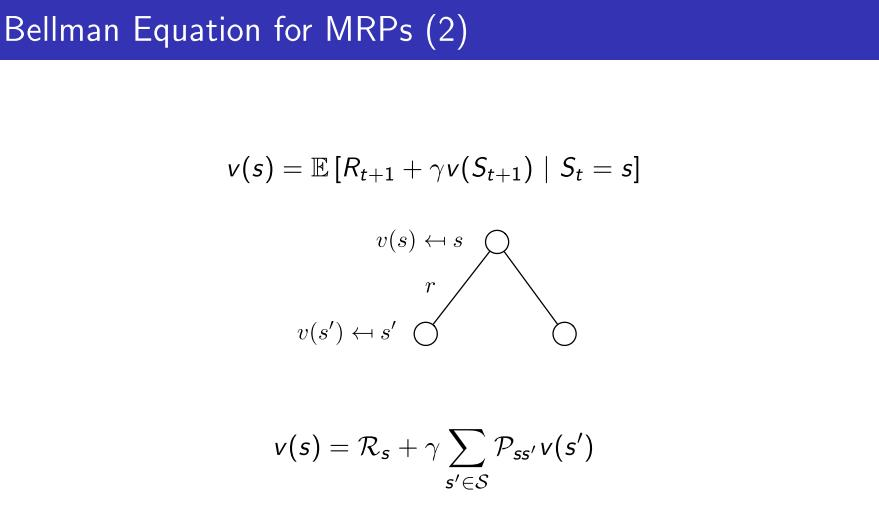
\includegraphics[width = \linewidth]{bellman.jpg}
	\end{centering}
\end{figure}

To express Bellman Equation in matrix form as $$v = R + \gamma P v,$$ we can solve Bellman Equation easily as linear equation.

\begin{equation*}
	\begin{aligned}[l]
		v &= R + \gamma P v \\
		(I - \gamma P)v &= R \\
		v &= (I - \gamma P)^{-1}R
	\end{aligned}•	
\end{equation*}•

%------------------------------------------------
% markov Decision process

\section{Markov Decision Process}
A MDP is a MRP with decisions, represented by a tuple $<S, A, P, R ,\gamma>$, 
to be specific, some params have been changed after action is introduced. 
$$P_{ss'}^a = \Bbb{P}[S_{t+1} = s' | S_{t} = s, A_{t} = a]$$ 
$$R^{a}_{s} = \Bbb{E}[R_{t+1} | S_{t} = s, A_{t} = a]$$

\subsection{Policies}

Policies: A policy $\pi$ is a distribution over actions given states, 
$$\pi(a|s) = \Bbb{P}[A_{t} = a | S_{t} = s]$$

\begin{itemize}
\item{A policy fully characterizes the agent's behaviour}
\item{Policy is what we want in RL problem}
\item{Policy is only asscoiated with current state}
\item{Policy is static if it's certain}
\item{Agent can update policy during the time}
\item{If $\pi$ is one-hot, then policy is certain}

\end{itemize}

\begin{figure}[h]
	\begin{centering}
		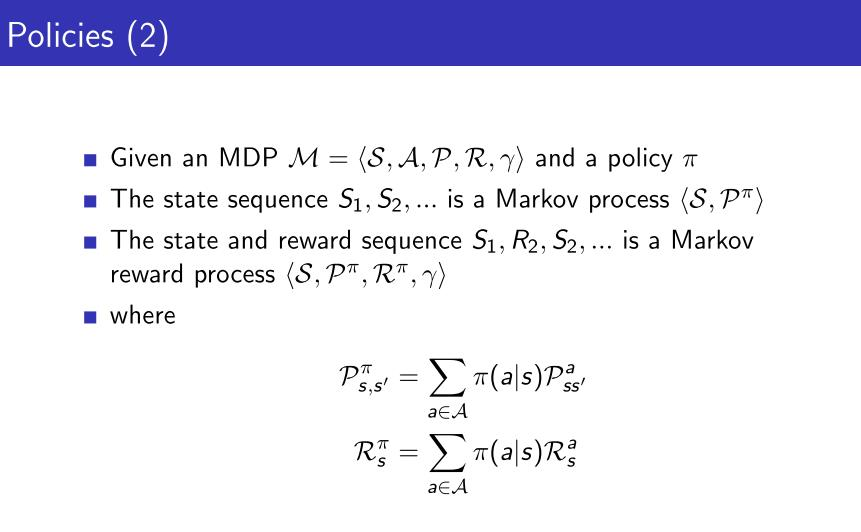
\includegraphics[width = \linewidth]{policy.jpg}
	\end{centering}
\end{figure}

After we introduce Policy, we should reinvent the value function.
the state-value funcion is:
$$v_{\pi}(s) = \Bbb{E}_{\pi}[G_{t} | S_{t} = s] $$
the action-value function is:
$$q_{\pi}(s, a) = \Bbb{E}_{\pi}[G_{t} | S_{t} = s, A_{t} = a] $$

\subsection{Bellman Expectation Equation}

\begin{figure}[H]
	\begin{centering}
		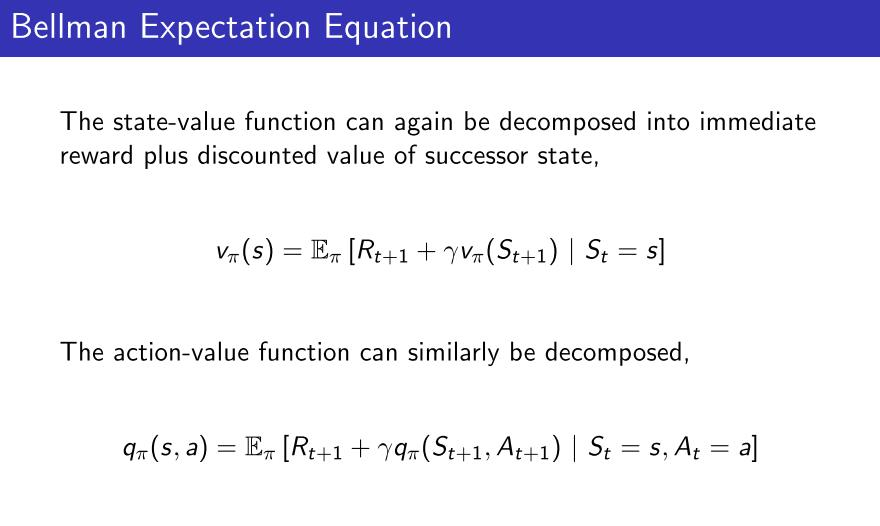
\includegraphics[width = \linewidth]{bellmanEE.jpg}
	\end{centering}
\end{figure}

\begin{figure}[H]
	\begin{centering}
		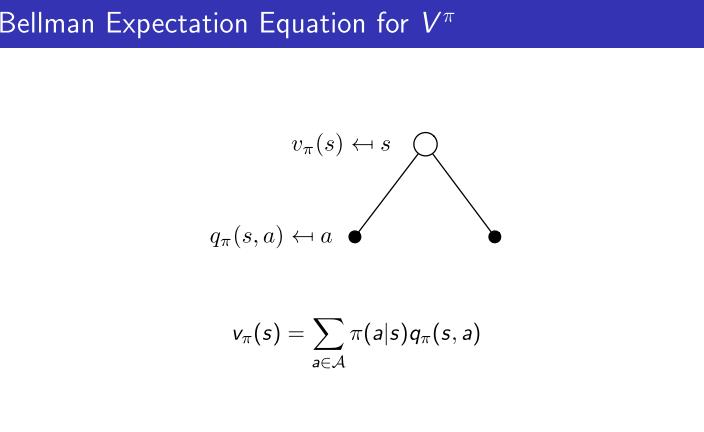
\includegraphics[width = \linewidth]{bellmanV.jpg}
	\end{centering}
\end{figure}

For each action nod, q-value is generated the same way.
\begin{figure}[H]
	\begin{centering}
		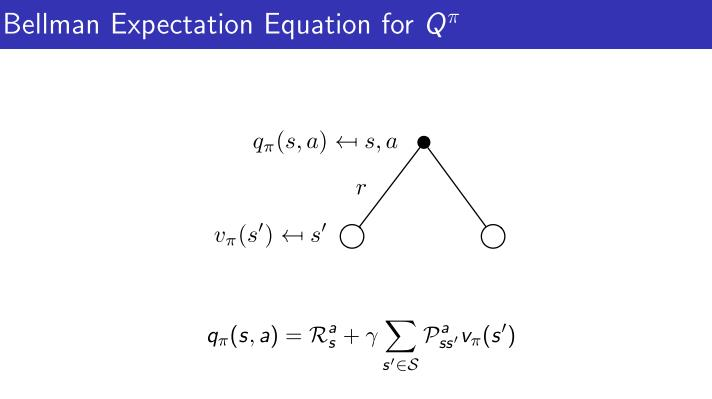
\includegraphics[width = \linewidth]{bellmanQ.jpg}
	\end{centering}
\end{figure}

Two process combined in various order, we can get Bellman Expectation Equation for $v_{\pi}$ and $q_{\pi}$

\begin{figure}[H]
	\begin{centering}
		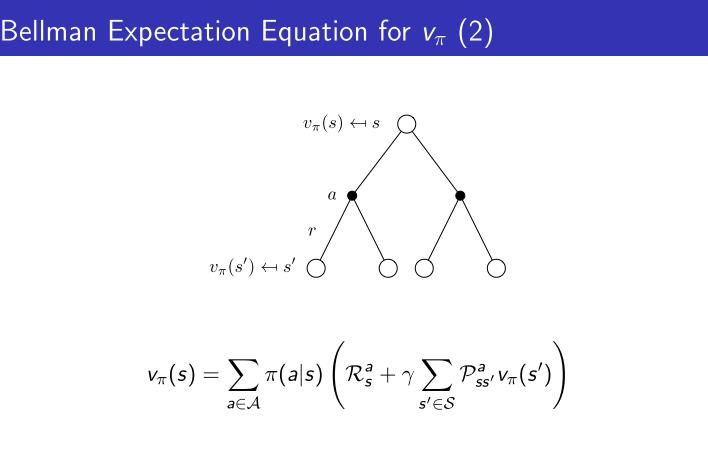
\includegraphics[width = \linewidth]{bellmanVpi.jpg}
	\end{centering}
\end{figure}

\begin{figure}[H]
	\begin{centering}
		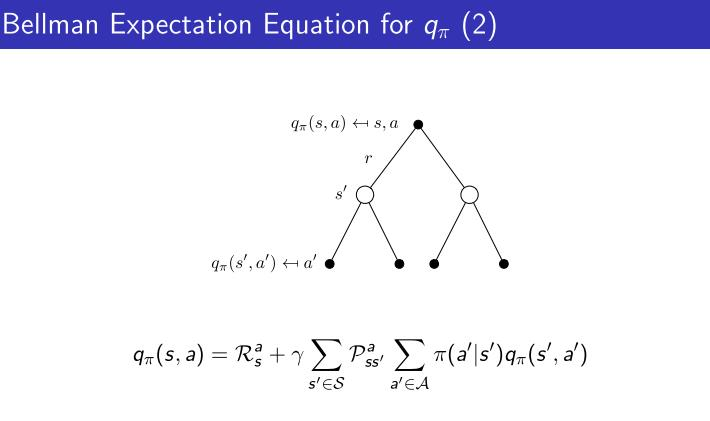
\includegraphics[width = \linewidth]{bellmanQpi.jpg}
	\end{centering}
\end{figure}

\subsection{Optimal Value Function}

\subsubsection{Definition}
The optimal state-value function $v_{*}(s)$ is the maximum value function over all policies
$$v_{*}(s) = \underset{\pi}\max \; v_{\pi}(s)$$

The optimal action-value function $q_{*}(s,a)$ is the maximum action-value function over all policies
$$ q_{*}(s,a) = \underset{\pi}\max \; q_{\pi}(s,a) $$

\subsubsection{Optimal Policy}
\begin{figure}[H]
	\begin{centering}
		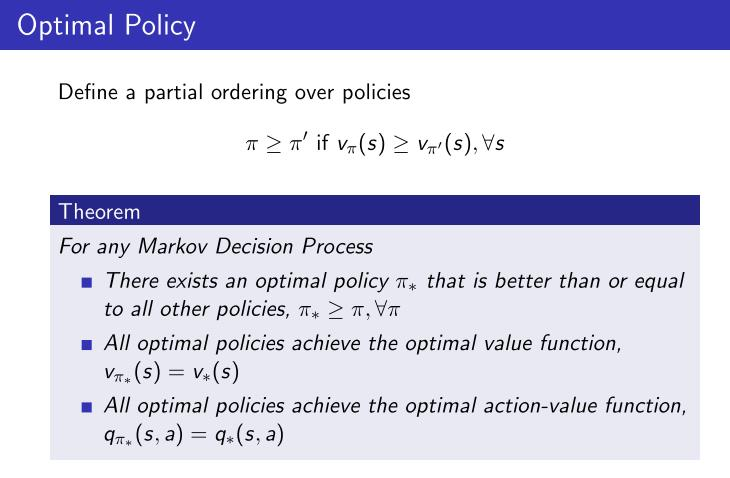
\includegraphics[width = \linewidth]{OptPolicy.jpg}
	\end{centering}
\end{figure}

\subsubsection{Find Optimal Policy}
\begin{figure}[H]
	\begin{centering}
		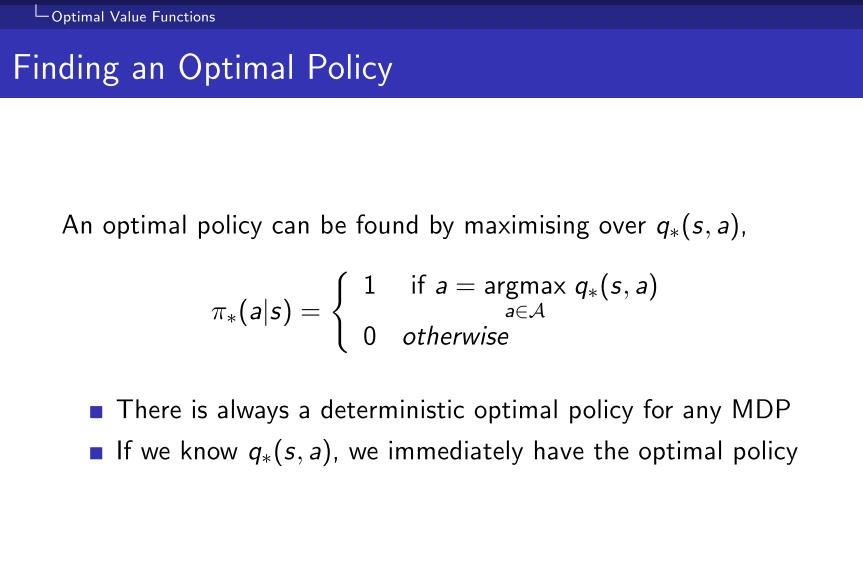
\includegraphics[width = \linewidth]{findopt.jpg}
	\end{centering}
\end{figure}

\subsection{Bellman Optimality Equation}

\begin{figure}[H]
	\begin{centering}
		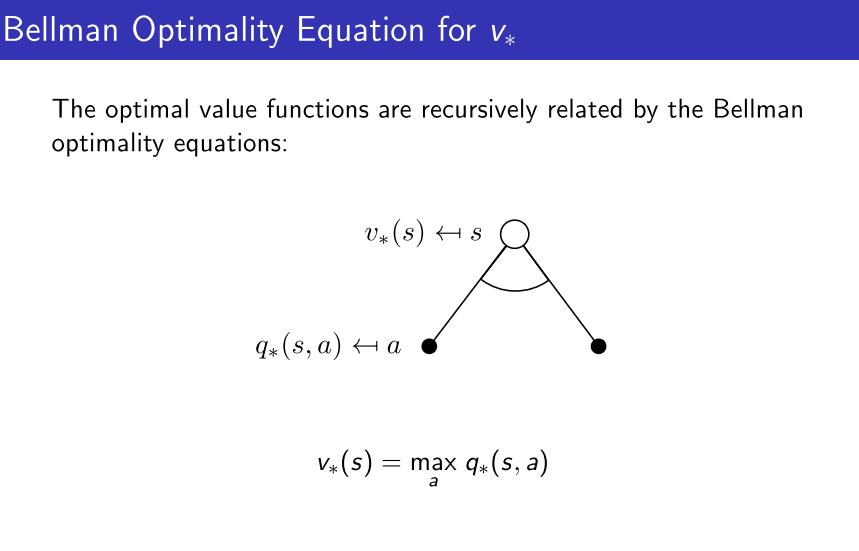
\includegraphics[width = \linewidth]{bellmanOptV.jpg}
	\end{centering}
\end{figure}

\begin{figure}[H]
	\begin{centering}
		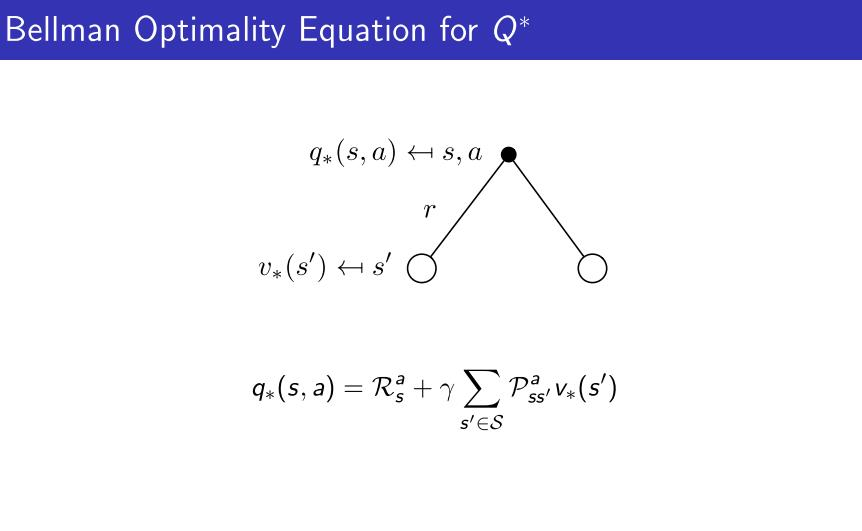
\includegraphics[width = \linewidth]{bellmanOptQ.jpg}
	\end{centering}
\end{figure}

\begin{figure}[H]
	\begin{centering}
		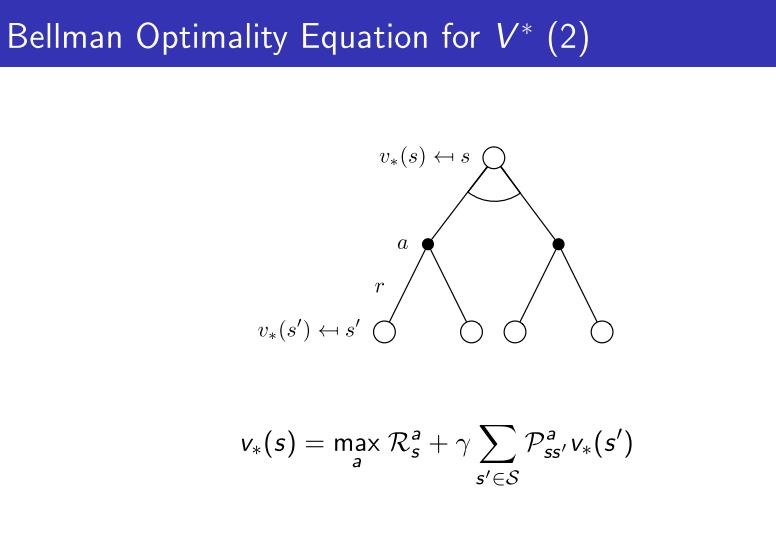
\includegraphics[width = \linewidth]{bellmanOptV2.jpg}
	\end{centering}
\end{figure}

\begin{figure}[H]
	\begin{centering}
		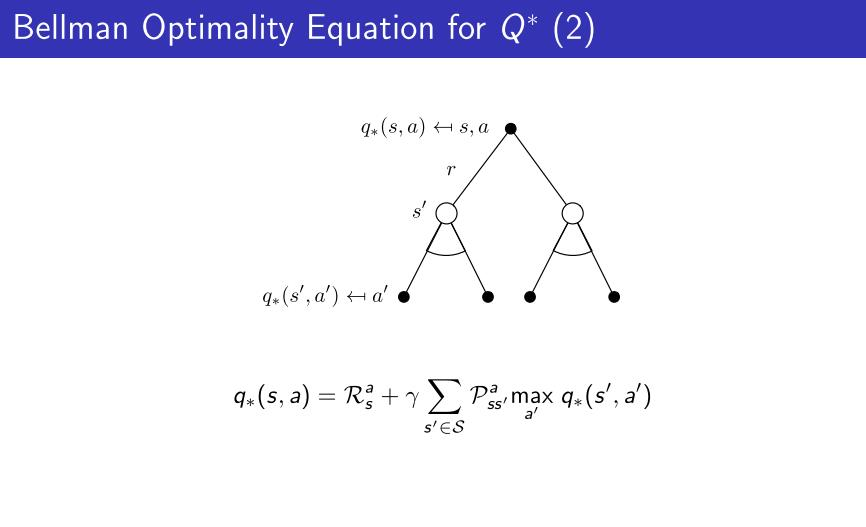
\includegraphics[width = \linewidth]{bellmanOptQ2.jpg}
	\end{centering}
\end{figure}

%------------------------------------------------
\section{Example Demonstration}
I import example from \citep{reference2} and explanation from \citep{reference1}, accompanied with my personal perspective to finish this part.

\subsection{MRP Example}
Given the following Markov Reward Process
\begin{figure}[H]
	\begin{centering}
		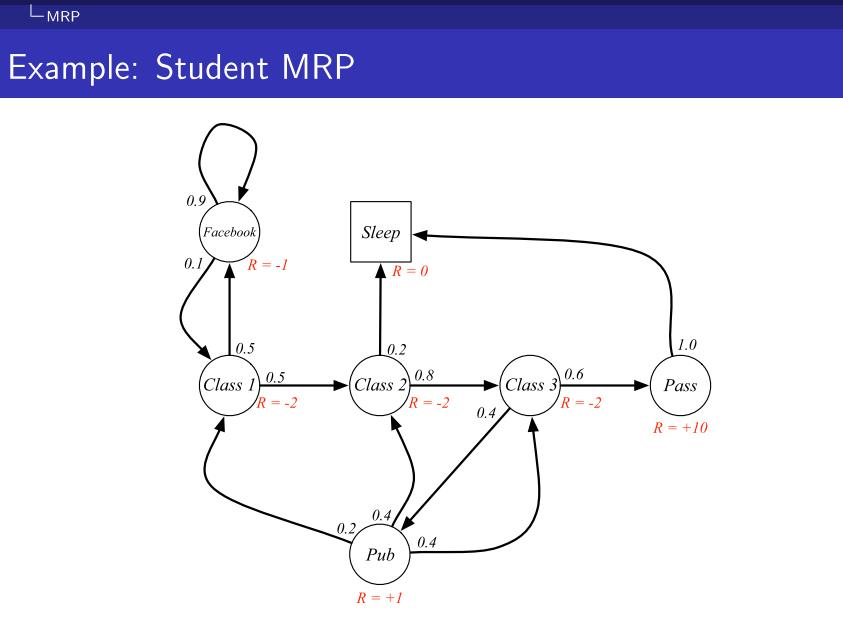
\includegraphics[width = \linewidth]{MRP.jpg}
	\end{centering}
\end{figure},
We can extract this process into a matrix:
\begin{align*}
	\begin{bmatrix}
		\begin{smallmatrix}
		\textbf{Reward} 	 & -1				& -2		 & -2			& -2 		 & 10		& 1		& 0\\
		\textbf{State}  	 & FaceBook	& Class1 & Class2 & Class3 & Pass & Pub & Sleep\\
		FaceBook & 0.9			& 0.1		 & 				&				 &			&			& \\
		Class1   & 0.5			&  			 & 0.5		&				 &			&			& \\
		Class2	 & 					& 			 & 				&	0.8		 &			&			& 0.2\\
		Class3	 & 					& 		 	 & 				&				 & 0.6	&	0.4	& \\
		Pass	   & 					& 		 	 & 				&				 &			&			& 1\\
		Pub			 & 					& 0.2	 	 & 0.4		&	0.4		 & 			&			& \\
		Sleep		 & 					& 		 	 & 				&				 &			&			& 1\\
		\end{smallmatrix}	
	\end{bmatrix}
\end{align*}

where 
\begin{align*}
	\cal{S} = 
	\begin{bmatrix}
		\begin{smallmatrix}
			FaceBook \\
			Class1 \\
			Class2 \\
			Class3 \\
			Pass\\
			Pub\\
			Sleep
		\end{smallmatrix}
	\end{bmatrix},
\end{align*}

\begin{align*}
	\cal{P} = 
	\begin{bmatrix}
		\begin{smallmatrix}
			0.9			& 0.1		 & 				&				 &			&			& \\
			0.5			&  			 & 0.5		&				 &			&			& \\
		 	& 			 & 				&	0.8		 &			&			& 0.2\\
			& 		 	 & 				&				 & 0.6	&	0.4	& \\
		 	& 		 	 & 				&				 &			&			& 1\\
			& 0.2	 	 & 0.4		&	0.4		 & 			&			& \\
		 	& 		 	 & 				&				 &			&			& 1\\
		\end{smallmatrix}
	\end{bmatrix}
\end{align*}

\begin{align*}
	\cal{R} = 
	\begin{bmatrix}
		\begin{smallmatrix}
			-1 \\
			-2 \\
			-2 \\
			-2 \\
			10 \\
			1\\
			0
		\end{smallmatrix}
	\end{bmatrix},
\end{align*}

$$\gamma \in [0,1] $$

where we can use these params to calculate state value $v(s)$ using bellman equation
\begin{align*}
	v &= (I - \gamma P)^{-1}R \\
		&= \left( 
		\begin{bmatrix}
			\begin{smallmatrix}
			1&0&0&0&0&0&0\\
			0&1&0&0&0&0&0\\
			0&0&1&0&0&0&0\\
			0&0&0&1&0&0&0\\
			0&0&0&0&1&0&0\\
			0&0&0&0&0&1&0\\
			0&0&0&0&0&0&1
			\end{smallmatrix}
		\end{bmatrix}
		- \gamma
		\begin{bmatrix}
			\begin{smallmatrix}
				0.9			& 0.1		 & 				&				 &			&			& \\
				0.5			&  			 & 0.5		&				 &			&			& \\
		 		& 			 & 				&	0.8		 &			&			& 0.2\\
				& 		 	 & 				&				 & 0.6	&	0.4	& \\
		 		& 		 	 & 				&				 &			&			& 1\\
				& 0.2	 	 & 0.4		&	0.4		 & 			&			& \\
		 		& 		 	 & 				&				 &			&			& 1\\
			\end{smallmatrix}
		\end{bmatrix}
		\right)^{-1}
		\begin{bmatrix}
			\begin{smallmatrix}
			-1 \\
			-2 \\
			-2 \\
			-2 \\
			10 \\
			1\\
			0
			\end{smallmatrix}
		\end{bmatrix}
\end{align*}

The result state-value vector is stored in $s$, shown in \ref{fig:MRPres}

\begin{figure}[H]
	\begin{centering}
		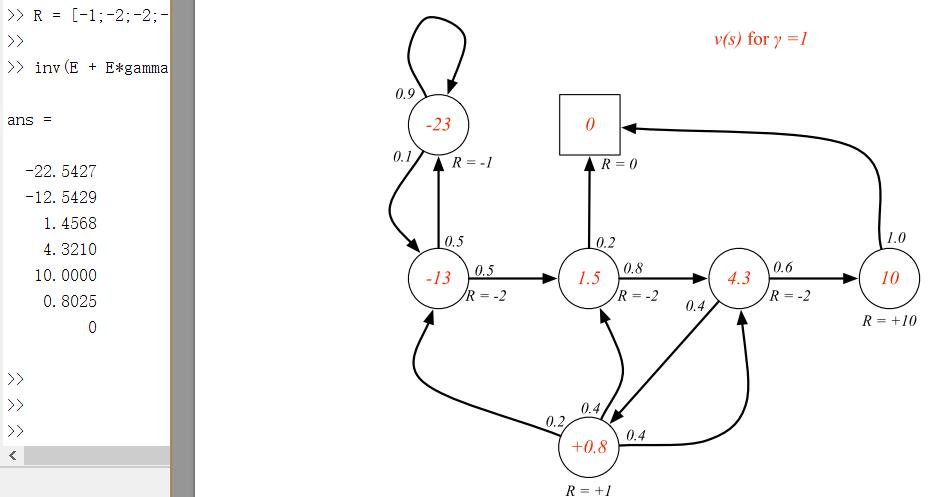
\includegraphics[width = \linewidth]{MRPexp.jpg}
	\end{centering}
	\caption{MRP results}
	\label{fig:MRPres}
\end{figure}

\subsection{MDP Example}
Introduce MDP example from the lecture.

\begin{figure}[H]
	\begin{centering}
		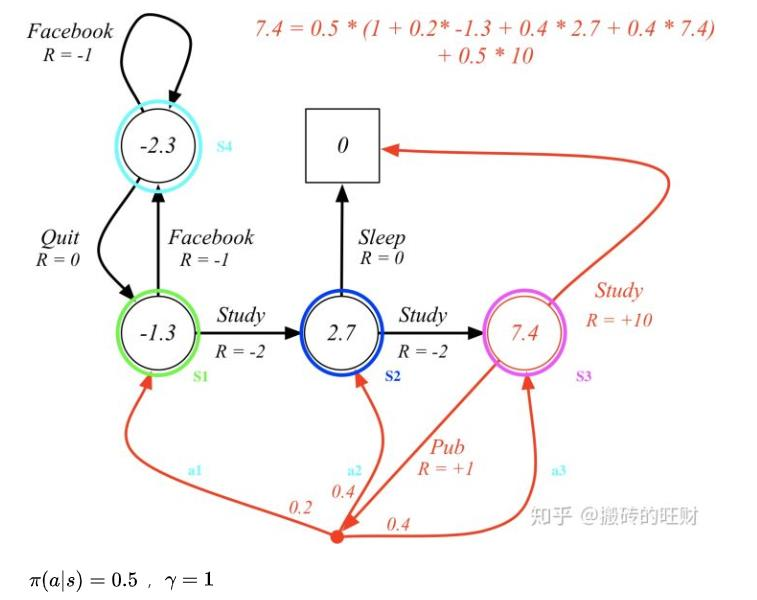
\includegraphics[width = \linewidth]{MDPexp.jpg}
	\end{centering}
\end{figure}

First, we can use state-value function to calculate the value of each state. Using 
$$v_{\pi}(s) = \sum_{a \in A} \pi(a|s) (R_{s}^a + \gamma \sum_{s'\in S} P^{a}_{s s^{'}} v_{\pi}(s^{'}))$$

since $\pi(a|s) = 0.5$, it means the decision is uniformly random. Also, the state value is initialized as zero-vector actually.
for $v(1)$, $$v(1) = 0.5*(-1 + v(4)) + 0.5*(-2 + v(2))$$

for $v(2)$, $$v(2) = 0.5*(-2 + v(3))$$

for $v(3)$, $$v(3) = 0.5*(10 + 0) + 0.5*(1 + (0.2*v(1) + 0.4*v(2) + 0.4*v(3))) $$

for $v(4)$, $$v(4) = 0.5*(-1 + v(4)) + 0.5*(0 + v(1))$$

From these four equations, we can calculate four state values.

\begin{align*}
	\begin{bmatrix}
			v1\\
			v2\\
			v3\\
			v4
	\end{bmatrix}
	=
	\begin{bmatrix}
		-1.3 \\
		2.7 \\
		7.4 \\
		-2.3 
	\end{bmatrix}
\end{align*}

After we have got state value, we can use the same method to obtain the value of action.

%----------------------------------------------------------------------------------------
%	BIBLIOGRAPHY
%----------------------------------------------------------------------------------------

\printbibliography[title={Reference}] % Print the bibliography, section title in curly brackets

%----------------------------------------------------------------------------------------

\end{document}
